%% bare_jrnl.tex
%% V1.4b
%% 2015/08/26
%% by Michael Shell
%% see http://www.michaelshell.org/
%% for current contact information.
%%
%% This is a skeleton file demonstrating the use of IEEEtran.cls
%% (requires IEEEtran.cls version 1.8b or later) with an IEEE
%% journal paper.
%%

\documentclass[journal,onecolumn]{IEEEtran}
%
% If IEEEtran.cls has not been installed into the LaTeX system files,
% manually specify the path to it like:
% \documentclass[journal]{../sty/IEEEtran}

\usepackage[pdftex]{graphicx}
\usepackage{amsmath}
\usepackage{algpseudocode}
\usepackage{algorithm}
\usepackage{cite}
%\usepackage{array}
%\usepackage[caption=false,font=normalsize,labelfont=sf,textfont=sf]{subfig}
%\usepackage{url}

\hyphenation{op-tical net-works semi-conduc-tor}

\begin{document}
% \title{_}
% \author{_}
% 
% \maketitle

\section{Methods}
%\IEEEPARstart{T}{his} 
This section explains two alternative methodologies to find moving flock patterns in large spatio-temporal datasets using modern distributed frameworks to divide and parallize the work load.

The first alternative follows closely the steps explained at \cite{vieira_-line_2009}.  At this work, the authors proposed the Basic Flock Evaluation (BFE) algorithm to find flock pattern on trajectories databases.  The details of the algorithm can be accessed at the source but figure \ref{fig:flowchart1} explains schematically the work flow where we can identify 4 general steps.

\begin{enumerate}
    \item Pair finding:  Using the $\varepsilon$ parameter, the algorithm query the set of points to get the set of pairs which laid at a maximum distance of $\varepsilon$ units.  Usually, it is a distance self-join operation over the set of points using $\varepsilon$ as the distance parameter.  The query also pays attention to do not return pair duplicates.  Pair between point $p_1$ and $p_2$ is the same that pair between $p_2$ and $p_1$ and just one of them should be reported (the id of each point is used to filter duplicates).
    \item Center computation:  From the set of pairs of points available, each tuple is the input of a simple computation to locate the centers of the two circles of radious $\frac{\varepsilon}{2}$ which circumference lied on the input points.  The pseudocode of the precedure can be seen in appendix \ref{app:centers}.
\end{enumerate}

\begin{figure}[b]
    \centering
    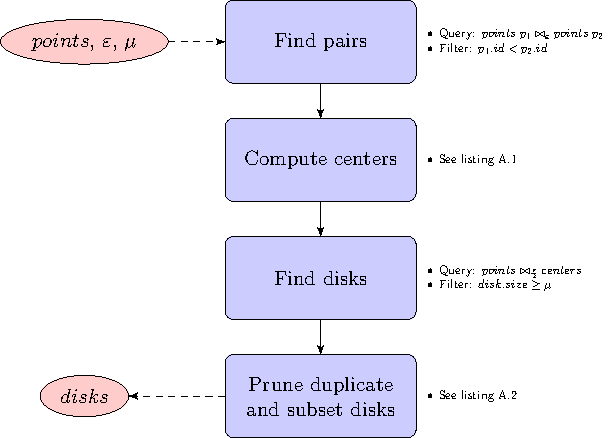
\includegraphics{figures/flowchart1}
    \caption{General steps in BFE algorithm.}\label{fig:flowchart1}
\end{figure}

\appendices
\section{Center computation.}\label{app:centers}
Appendix one explains center computation.

\alglanguage{pseudocode}
\begin{algorithm}
\caption{A small pseudocode}
\begin{algorithmic}[1]
\State $s \gets 0$
\State $p \gets 0$
\For{$i \gets 1,\, 10$}
\State $s \gets s + i$
\State $p \gets p + s$
\EndFor
\end{algorithmic}
\end{algorithm}

\section{Disk prunning.}\label{app:disks}
Appendix two explains disk prunning.

\bibliographystyle{IEEEtran}
\bibliography{../pflocks.bib}



\end{document}
